\chapter{Implementasi dan Pengujian}
\label{chap:implementasiPengujian}

Bab ini terdiri atas dua bagian, yaitu Implementasi Perangkat Lunak dan Pengujian Perangkat Lunak. Bagian implementasi berisi penjelasan lingkungan pengembangan perangkat lunak dan hasil implementasi. Sedangkan bagian pengujian berisi hasil pengujian fungsional dan eksperimental terhadap perangkat lunak yang telah dibangun.

\section{Implementasi}
\label{sec:implementasi}

\subsection{Lingkungan Implementasi}
\label{sec:lingkungan_implementasi}
Implementasi perangkat lunak ini dilakukan di komputer dengan spesifikasi sebagai berikut:
\begin{enumerate}
	\item Processor: 1.6 GHz
	\item RAM: 4 GB 1600 MHz DDR3
	\item Sistem Operasi: OS X Yosemite version 10.10.5
	\item Versi Java: 1.8.0\_51
\end{enumerate}

\subsection{Hasil Implementasi}
Hasil implementasi berupa aplikasi berbasis web yang menggunakan Play Framework. Aplikasi dapat diakses pada jaringan lokal dengan URL \url{localhost:9000}. Aplikasi KIRI terdiri dari satu halaman utama. Halaman utama KIRI, pengguna dapat melakukan pencarian rute KIRI dengan masukan nama tempat atau masukan berupa klik pada peta yang disediakan pada halaman utama KIRI. Setelah melakukan masukan untuk pencarian rute, muncul hasil pencarian rute dan/atau hasil alternatif rute yang ditampilkan pada halaman utama KIRI serta menggambarkan hasil rute pada peta yang disediakan aplikasi KIRI.

\begin{figure}[H]
	\centering
	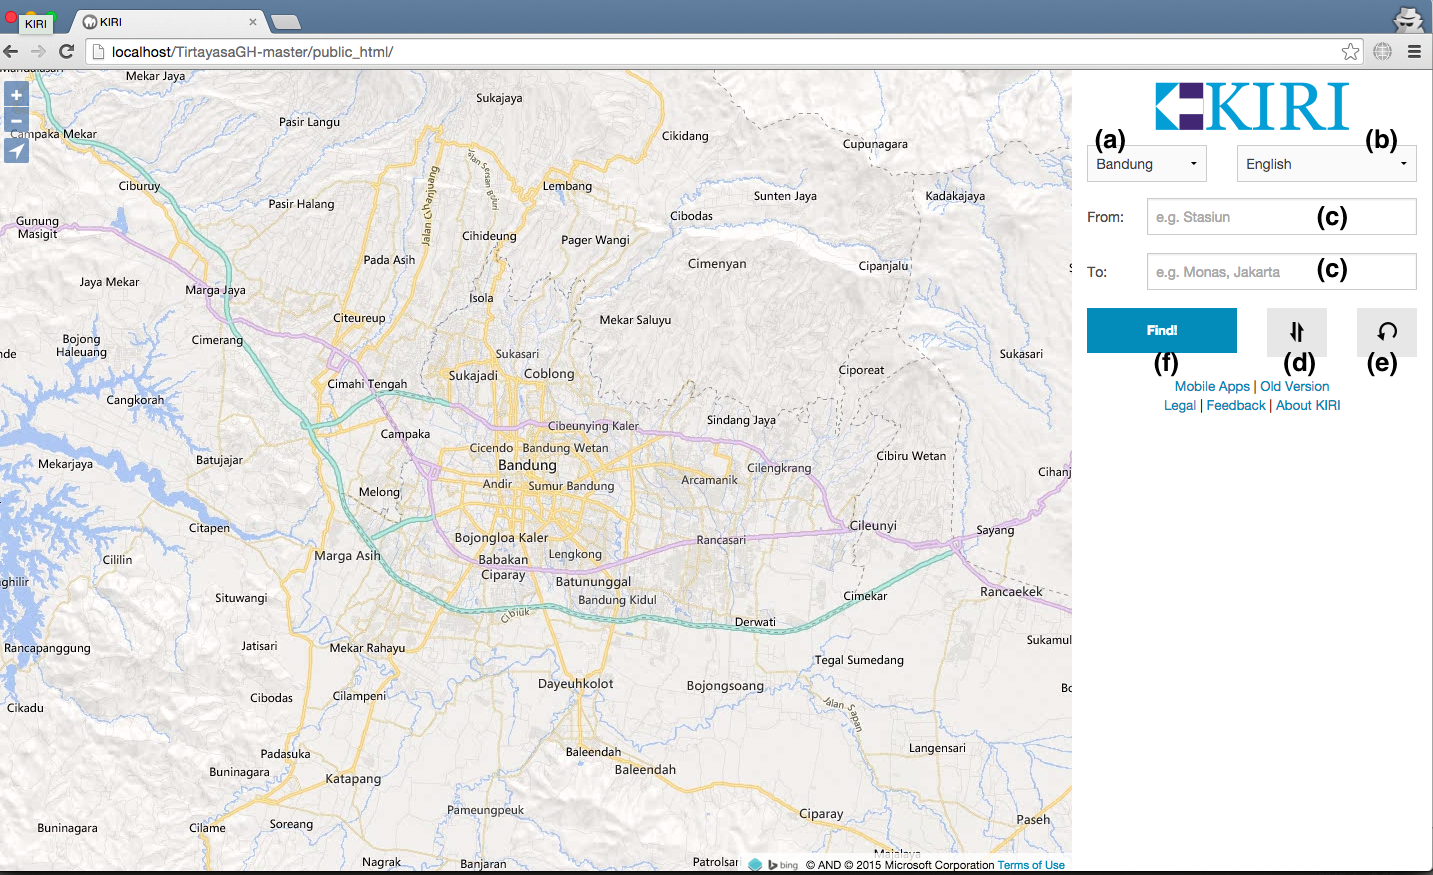
\includegraphics[scale=0.3]{Gambar/KIRI-main}
	\caption{Halaman Utama KIRI} 
	\label{fig:5_KIRI_main}
\end{figure}


\begin{figure}[H]
	\centering
	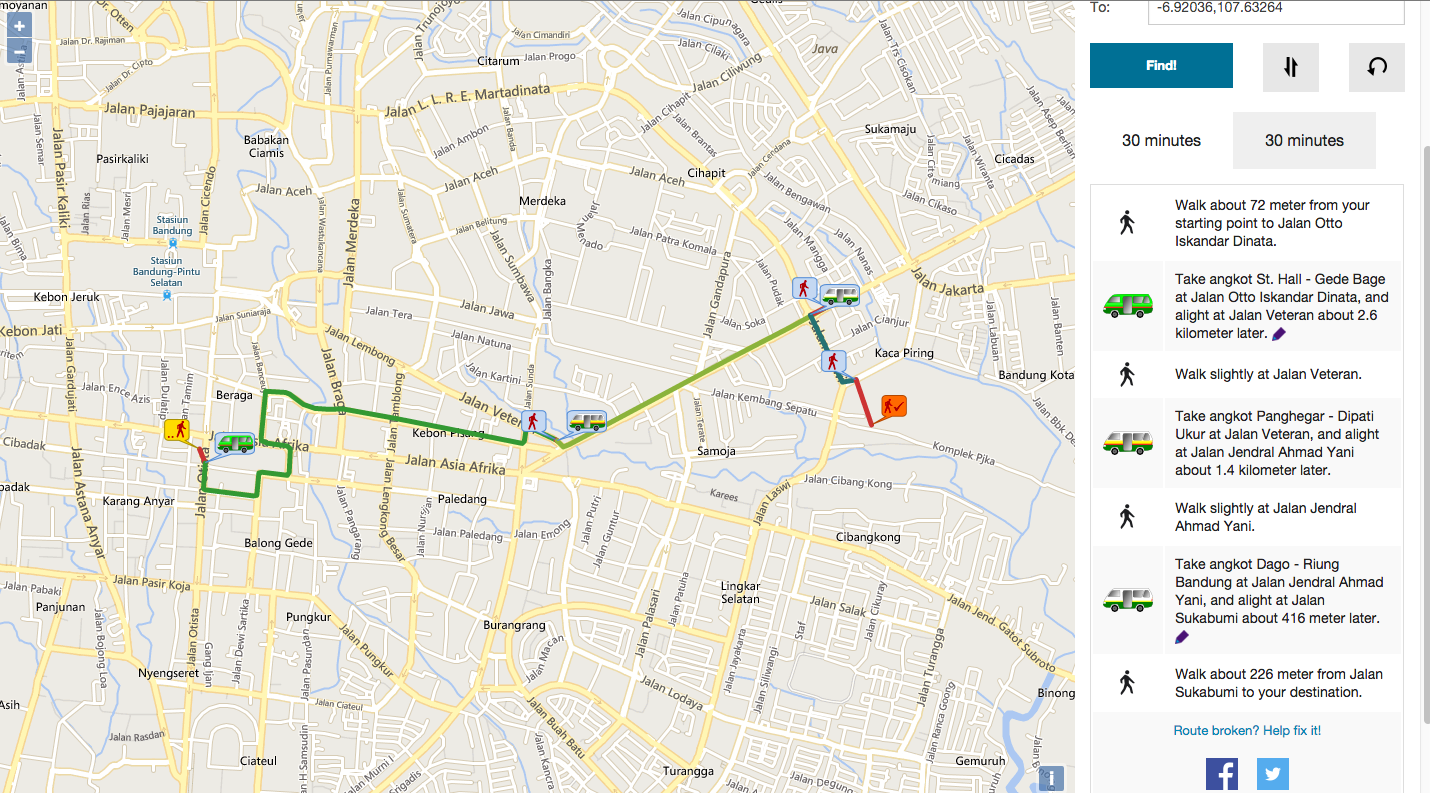
\includegraphics[scale=0.3]{Gambar/KIRI-find}
	\caption{Contoh Pencarian Rute pada KIRI} 
	\label{fig:5_KIRI_find}
\end{figure}

\begin{figure}[H]
	\centering
	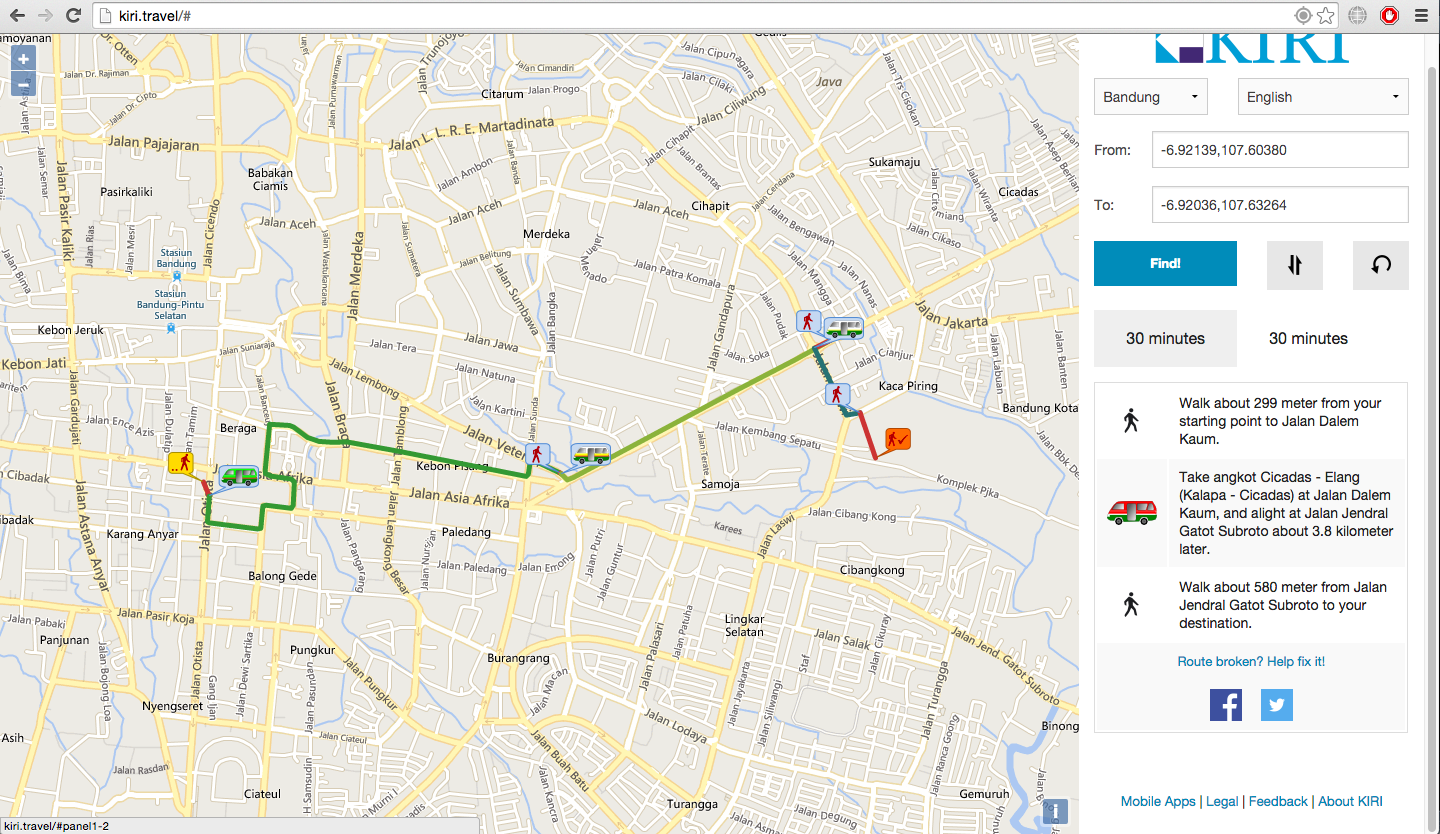
\includegraphics[scale=0.3]{Gambar/KIRI-find-alternate}
	\caption{Contoh Rute Alternatif pada KIRI} 
	\label{fig:5_KIRI_find_alternate}
\end{figure}

\section{Pengujian}
\subsection{Pengujian Fungsional}

Pengujian fungsional dilakukan untuk mengetahui kesesuaian reaksi perangkat lunak dengan reaksi yang diharapkan berdasarkan aksi pengguna terhadap perangkat lunak. Pengujian ini dilakukan pada berbagai sistem yaitu Windows, Linux, MacOS, dan Android dengan hasil yang sama. Terdapat tujuh tes kasus yang diujikan, detail serta hasilnya dapat dilihat pada Tabel \ref{table:hasilFungsional}.
			
\begin{table}[H]
	\centering
	\caption{Tabel Pengujian Fungsional}
		\begin{tabular}{|p{0.25cm}| p{3.5cm}| p{7cm}| p{2.5cm}|} \hline
		No.	&	Aksi Pengguna	&	Reaksi yang diharapkan	&	Reaksi Perangkat Lunak \\ \hline
		1.	&	Pengguna menjalankan aplikasi	&	Halaman utama akan ditampilkan	&	sesuai	\\ \hline
		
		\end{tabular}
	\label{table:hasilFungsional}
\end{table}